\documentclass[twoside]{book}

% Packages required by doxygen
\usepackage{fixltx2e}
\usepackage{calc}
\usepackage{doxygen}
\usepackage[export]{adjustbox} % also loads graphicx
\usepackage{graphicx}
\usepackage[utf8]{inputenc}
\usepackage{makeidx}
\usepackage{multicol}
\usepackage{multirow}
\PassOptionsToPackage{warn}{textcomp}
\usepackage{textcomp}
\usepackage[nointegrals]{wasysym}
\usepackage[table]{xcolor}

% Font selection
\usepackage[T1]{fontenc}
\usepackage[scaled=.90]{helvet}
\usepackage{courier}
\usepackage{amssymb}
\usepackage{sectsty}
\renewcommand{\familydefault}{\sfdefault}
\allsectionsfont{%
  \fontseries{bc}\selectfont%
  \color{darkgray}%
}
\renewcommand{\DoxyLabelFont}{%
  \fontseries{bc}\selectfont%
  \color{darkgray}%
}
\newcommand{\+}{\discretionary{\mbox{\scriptsize$\hookleftarrow$}}{}{}}

% Page & text layout
\usepackage{geometry}
\geometry{%
  a4paper,%
  top=2.5cm,%
  bottom=2.5cm,%
  left=2.5cm,%
  right=2.5cm%
}
\tolerance=750
\hfuzz=15pt
\hbadness=750
\setlength{\emergencystretch}{15pt}
\setlength{\parindent}{0cm}
\setlength{\parskip}{3ex plus 2ex minus 2ex}
\makeatletter
\renewcommand{\paragraph}{%
  \@startsection{paragraph}{4}{0ex}{-1.0ex}{1.0ex}{%
    \normalfont\normalsize\bfseries\SS@parafont%
  }%
}
\renewcommand{\subparagraph}{%
  \@startsection{subparagraph}{5}{0ex}{-1.0ex}{1.0ex}{%
    \normalfont\normalsize\bfseries\SS@subparafont%
  }%
}
\makeatother

% Headers & footers
\usepackage{fancyhdr}
\pagestyle{fancyplain}
\fancyhead[LE]{\fancyplain{}{\bfseries\thepage}}
\fancyhead[CE]{\fancyplain{}{}}
\fancyhead[RE]{\fancyplain{}{\bfseries\leftmark}}
\fancyhead[LO]{\fancyplain{}{\bfseries\rightmark}}
\fancyhead[CO]{\fancyplain{}{}}
\fancyhead[RO]{\fancyplain{}{\bfseries\thepage}}
\fancyfoot[LE]{\fancyplain{}{}}
\fancyfoot[CE]{\fancyplain{}{}}
\fancyfoot[RE]{\fancyplain{}{\bfseries\scriptsize Generated by Doxygen }}
\fancyfoot[LO]{\fancyplain{}{\bfseries\scriptsize Generated by Doxygen }}
\fancyfoot[CO]{\fancyplain{}{}}
\fancyfoot[RO]{\fancyplain{}{}}
\renewcommand{\footrulewidth}{0.4pt}
\renewcommand{\chaptermark}[1]{%
  \markboth{#1}{}%
}
\renewcommand{\sectionmark}[1]{%
  \markright{\thesection\ #1}%
}

% Indices & bibliography
\usepackage{natbib}
\usepackage[titles]{tocloft}
\setcounter{tocdepth}{3}
\setcounter{secnumdepth}{5}
\makeindex

% Hyperlinks (required, but should be loaded last)
\usepackage{ifpdf}
\ifpdf
  \usepackage[pdftex,pagebackref=true]{hyperref}
\else
  \usepackage[ps2pdf,pagebackref=true]{hyperref}
\fi
\hypersetup{%
  colorlinks=true,%
  linkcolor=blue,%
  citecolor=blue,%
  unicode%
}

% Custom commands
\newcommand{\clearemptydoublepage}{%
  \newpage{\pagestyle{empty}\cleardoublepage}%
}

\usepackage{caption}
\captionsetup{labelsep=space,justification=centering,font={bf},singlelinecheck=off,skip=4pt,position=top}

%===== C O N T E N T S =====

\begin{document}

% Titlepage & ToC
\hypersetup{pageanchor=false,
             bookmarksnumbered=true,
             pdfencoding=unicode
            }
\pagenumbering{roman}
\begin{titlepage}
\vspace*{7cm}
\begin{center}%
{\Large My Project }\\
\vspace*{1cm}
{\large Generated by Doxygen 1.8.11}\\
\end{center}
\end{titlepage}
\clearemptydoublepage
\tableofcontents
\clearemptydoublepage
\pagenumbering{arabic}
\hypersetup{pageanchor=true}

%--- Begin generated contents ---
\chapter{Hierarchical Index}
\section{Class Hierarchy}
This inheritance list is sorted roughly, but not completely, alphabetically\+:\begin{DoxyCompactList}
\item Q\+Main\+Window\begin{DoxyCompactList}
\item \contentsline{section}{Main\+Window}{\pageref{classMainWindow}}{}
\end{DoxyCompactList}
\item Q\+Object\begin{DoxyCompactList}
\item \contentsline{section}{Bluetooth\+Client}{\pageref{classBluetoothClient}}{}
\item \contentsline{section}{Bluetooth\+Server}{\pageref{classBluetoothServer}}{}
\item \contentsline{section}{Client\+SC}{\pageref{classClientSC}}{}
\item \contentsline{section}{Frame3D}{\pageref{classFrame3D}}{}
\item \contentsline{section}{Server\+SC}{\pageref{classServerSC}}{}
\end{DoxyCompactList}
\item Q\+Window\begin{DoxyCompactList}
\item \contentsline{section}{Window}{\pageref{classWindow}}{}
\end{DoxyCompactList}
\end{DoxyCompactList}

\chapter{Class Index}
\subsection{Class List}
Here are the classes, structs, unions and interfaces with brief descriptions\+:\begin{DoxyCompactList}
\item\contentsline{section}{\hyperlink{class_memgrp___test}{Memgrp\+\_\+\+Test} \\*A class }{\pageref{class_memgrp___test}}{}
\end{DoxyCompactList}

\chapter{Class Documentation}
\hypertarget{classBluetoothClient}{}\section{Bluetooth\+Client Class Reference}
\label{classBluetoothClient}\index{Bluetooth\+Client@{Bluetooth\+Client}}
Inheritance diagram for Bluetooth\+Client\+:\begin{figure}[H]
\begin{center}
\leavevmode
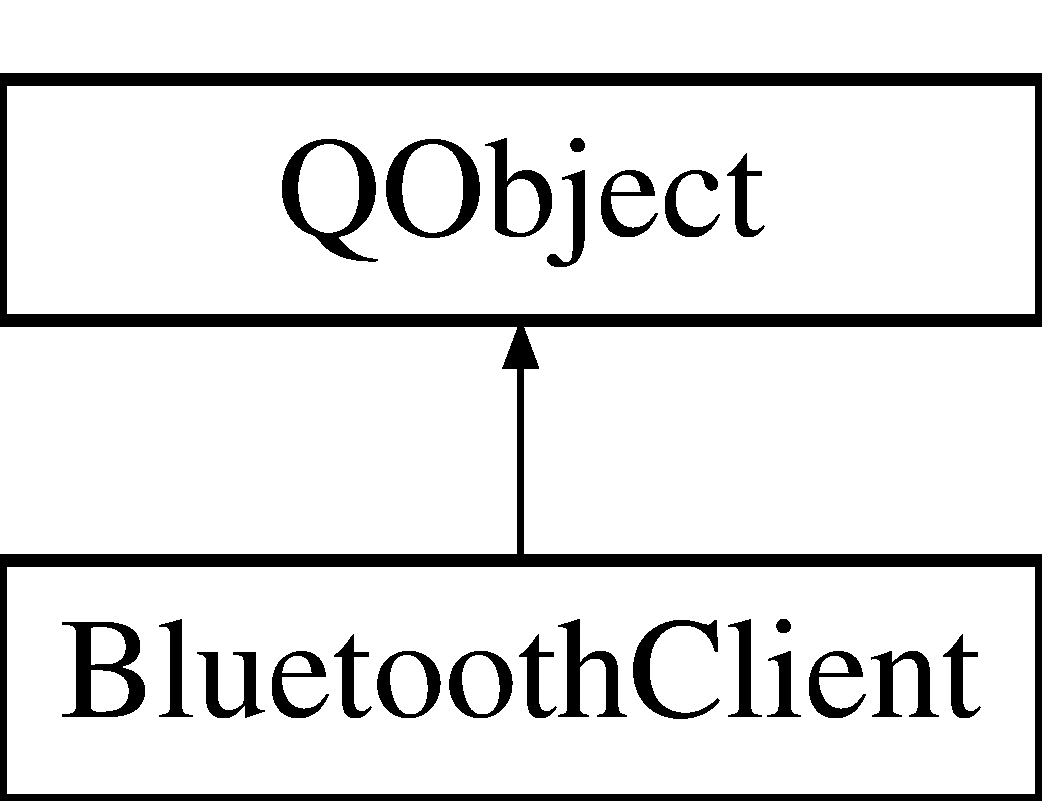
\includegraphics[height=2.000000cm]{classBluetoothClient}
\end{center}
\end{figure}
\subsection*{Public Slots}
\begin{DoxyCompactItemize}
\item 
void \hyperlink{classBluetoothClient_a698d488b94e8d0e866620130cf865aad}{send\+Message} (const Q\+String \&message)
\begin{DoxyCompactList}\small\item\em \mbox{[}Slot\mbox{]} used to send a message \end{DoxyCompactList}\end{DoxyCompactItemize}
\subsection*{Signals}
\begin{DoxyCompactItemize}
\item 
void \hyperlink{classBluetoothClient_a6cb91adb86f0a8ec6e378f721b6710a5}{message\+Received} (const Q\+String \&sender, const Q\+String \&message)
\begin{DoxyCompactList}\small\item\em \mbox{[}Signal\mbox{]} a message has been received by sender \end{DoxyCompactList}\item 
void \hyperlink{classBluetoothClient_ae1bc0e1cb03c8f3affb3cfb12a2aa328}{connected} (const Q\+String \&name)
\begin{DoxyCompactList}\small\item\em The client is connected. \end{DoxyCompactList}\item 
void \hyperlink{classBluetoothClient_a60a0cd485da3beee051c8fea6c788834}{disconnected} ()\hypertarget{classBluetoothClient_a60a0cd485da3beee051c8fea6c788834}{}\label{classBluetoothClient_a60a0cd485da3beee051c8fea6c788834}

\begin{DoxyCompactList}\small\item\em The client is disconnected from server. \end{DoxyCompactList}\end{DoxyCompactItemize}
\subsection*{Public Member Functions}
\begin{DoxyCompactItemize}
\item 
\hyperlink{classBluetoothClient_a5ee534b5d9823be1e297f037c50beaf6}{Bluetooth\+Client} ()\hypertarget{classBluetoothClient_a5ee534b5d9823be1e297f037c50beaf6}{}\label{classBluetoothClient_a5ee534b5d9823be1e297f037c50beaf6}

\begin{DoxyCompactList}\small\item\em \hyperlink{classBluetoothClient}{Bluetooth\+Client} constructor. \end{DoxyCompactList}\item 
void \hyperlink{classBluetoothClient_a478158ca1a19982dcccd0da4d60c4355}{start\+Client} (const Q\+Bluetooth\+Service\+Info \&remote\+Service)
\begin{DoxyCompactList}\small\item\em Establish connection with the service in bluetooth thanks to a socket. \end{DoxyCompactList}\item 
void \hyperlink{classBluetoothClient_ac2686da0bdb51fab22776ad68a6d7278}{stop\+Client} ()\hypertarget{classBluetoothClient_ac2686da0bdb51fab22776ad68a6d7278}{}\label{classBluetoothClient_ac2686da0bdb51fab22776ad68a6d7278}

\begin{DoxyCompactList}\small\item\em close the connection \end{DoxyCompactList}\end{DoxyCompactItemize}


\subsection{Member Function Documentation}
\index{Bluetooth\+Client@{Bluetooth\+Client}!connected@{connected}}
\index{connected@{connected}!Bluetooth\+Client@{Bluetooth\+Client}}
\subsubsection[{\texorpdfstring{connected}{connected}}]{\setlength{\rightskip}{0pt plus 5cm}void Bluetooth\+Client\+::connected (
\begin{DoxyParamCaption}
\item[{const Q\+String \&}]{name}
\end{DoxyParamCaption}
)\hspace{0.3cm}{\ttfamily [signal]}}\hypertarget{classBluetoothClient_ae1bc0e1cb03c8f3affb3cfb12a2aa328}{}\label{classBluetoothClient_ae1bc0e1cb03c8f3affb3cfb12a2aa328}


The client is connected. 


\begin{DoxyParams}{Parameters}
{\em name} & \+: server name \\
\hline
\end{DoxyParams}
\index{Bluetooth\+Client@{Bluetooth\+Client}!message\+Received@{message\+Received}}
\index{message\+Received@{message\+Received}!Bluetooth\+Client@{Bluetooth\+Client}}
\subsubsection[{\texorpdfstring{message\+Received}{messageReceived}}]{\setlength{\rightskip}{0pt plus 5cm}void Bluetooth\+Client\+::message\+Received (
\begin{DoxyParamCaption}
\item[{const Q\+String \&}]{sender, }
\item[{const Q\+String \&}]{message}
\end{DoxyParamCaption}
)\hspace{0.3cm}{\ttfamily [signal]}}\hypertarget{classBluetoothClient_a6cb91adb86f0a8ec6e378f721b6710a5}{}\label{classBluetoothClient_a6cb91adb86f0a8ec6e378f721b6710a5}


\mbox{[}Signal\mbox{]} a message has been received by sender 


\begin{DoxyParams}{Parameters}
{\em sender} & \\
\hline
{\em message} & \\
\hline
\end{DoxyParams}
\index{Bluetooth\+Client@{Bluetooth\+Client}!send\+Message@{send\+Message}}
\index{send\+Message@{send\+Message}!Bluetooth\+Client@{Bluetooth\+Client}}
\subsubsection[{\texorpdfstring{send\+Message}{sendMessage}}]{\setlength{\rightskip}{0pt plus 5cm}void Bluetooth\+Client\+::send\+Message (
\begin{DoxyParamCaption}
\item[{const Q\+String \&}]{message}
\end{DoxyParamCaption}
)\hspace{0.3cm}{\ttfamily [slot]}}\hypertarget{classBluetoothClient_a698d488b94e8d0e866620130cf865aad}{}\label{classBluetoothClient_a698d488b94e8d0e866620130cf865aad}


\mbox{[}Slot\mbox{]} used to send a message 


\begin{DoxyParams}{Parameters}
{\em message} & \\
\hline
\end{DoxyParams}
\index{Bluetooth\+Client@{Bluetooth\+Client}!start\+Client@{start\+Client}}
\index{start\+Client@{start\+Client}!Bluetooth\+Client@{Bluetooth\+Client}}
\subsubsection[{\texorpdfstring{start\+Client(const Q\+Bluetooth\+Service\+Info \&remote\+Service)}{startClient(const QBluetoothServiceInfo &remoteService)}}]{\setlength{\rightskip}{0pt plus 5cm}void Bluetooth\+Client\+::start\+Client (
\begin{DoxyParamCaption}
\item[{const Q\+Bluetooth\+Service\+Info \&}]{remote\+Service}
\end{DoxyParamCaption}
)}\hypertarget{classBluetoothClient_a478158ca1a19982dcccd0da4d60c4355}{}\label{classBluetoothClient_a478158ca1a19982dcccd0da4d60c4355}


Establish connection with the service in bluetooth thanks to a socket. 


\begin{DoxyParams}{Parameters}
{\em remote\+Service} & \\
\hline
\end{DoxyParams}


The documentation for this class was generated from the following files\+:\begin{DoxyCompactItemize}
\item 
bluetoothclient.\+h\item 
bluetoothclient.\+cpp\end{DoxyCompactItemize}

\hypertarget{classBluetoothServer}{}\section{Bluetooth\+Server Class Reference}
\label{classBluetoothServer}\index{Bluetooth\+Server@{Bluetooth\+Server}}
Inheritance diagram for Bluetooth\+Server\+:\begin{figure}[H]
\begin{center}
\leavevmode
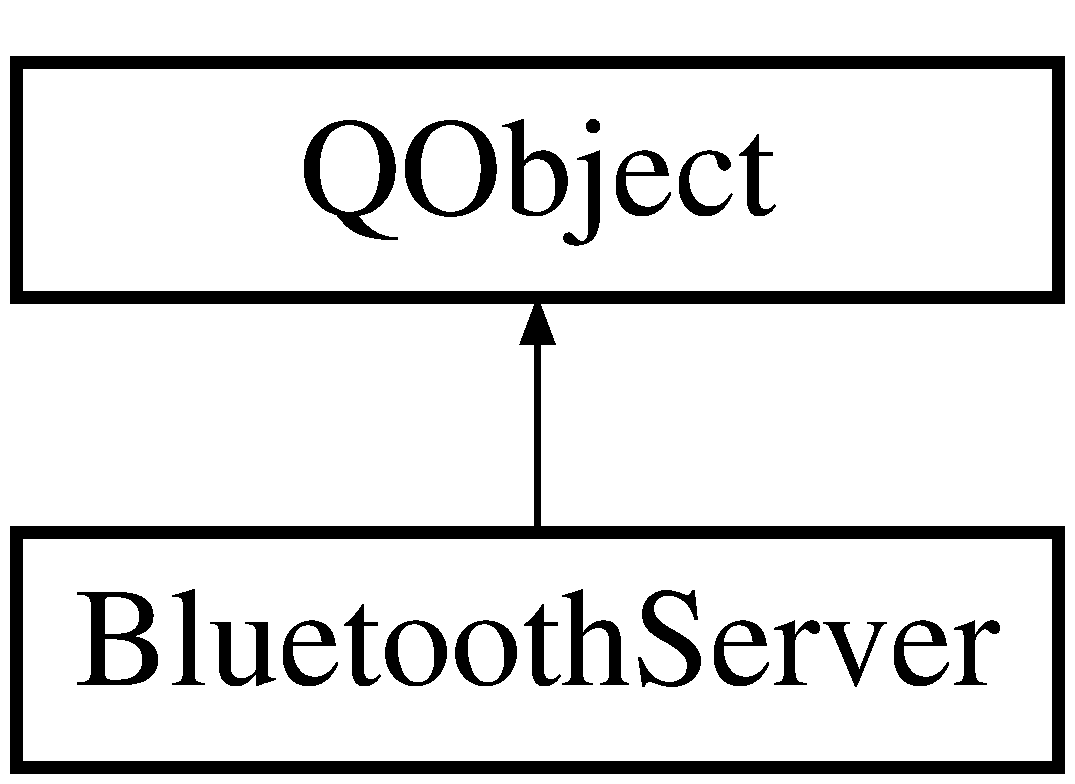
\includegraphics[height=2.000000cm]{classBluetoothServer}
\end{center}
\end{figure}
\subsection*{Public Slots}
\begin{DoxyCompactItemize}
\item 
void \hyperlink{classBluetoothServer_ab4b42cafe04f9b2d50abfd4f0b2986e9}{send\+Message} (const Q\+String \&message)
\begin{DoxyCompactList}\small\item\em \mbox{[}Slot\mbox{]} Used to send message through bluetooth \end{DoxyCompactList}\end{DoxyCompactItemize}
\subsection*{Signals}
\begin{DoxyCompactItemize}
\item 
void \hyperlink{classBluetoothServer_a743a58193190ac6d05845c0ff7430c8c}{s\+\_\+\+Client\+Connected} ()\hypertarget{classBluetoothServer_a743a58193190ac6d05845c0ff7430c8c}{}\label{classBluetoothServer_a743a58193190ac6d05845c0ff7430c8c}

\begin{DoxyCompactList}\small\item\em Signal emitted when a client is connected. \end{DoxyCompactList}\item 
void \hyperlink{classBluetoothServer_a2083b480c0816480d4835befe663cf1f}{error} (Q\+String)\hypertarget{classBluetoothServer_a2083b480c0816480d4835befe663cf1f}{}\label{classBluetoothServer_a2083b480c0816480d4835befe663cf1f}

\begin{DoxyCompactList}\small\item\em Signal used to explain the error that ocurred. \end{DoxyCompactList}\item 
void \hyperlink{classBluetoothServer_a4133b36b414c0ce886632a93cc29b735}{message\+Received} (const Q\+String \&sender, const Q\+String \&message)
\begin{DoxyCompactList}\small\item\em Signal emitted when a message is received. \end{DoxyCompactList}\item 
void \hyperlink{classBluetoothServer_a18b236c59af04e7439d77a48633350e8}{client\+Connected} (const Q\+String \&name)
\begin{DoxyCompactList}\small\item\em Signal emitted when a clien is connected to the server. \end{DoxyCompactList}\item 
void \hyperlink{classBluetoothServer_a17521320ad9e77537843c7d416e94bef}{client\+Disconnected} (const Q\+String \&name)
\begin{DoxyCompactList}\small\item\em Signal emitted when a client disconnects from the server. \end{DoxyCompactList}\end{DoxyCompactItemize}
\subsection*{Public Member Functions}
\begin{DoxyCompactItemize}
\item 
\hyperlink{classBluetoothServer_adfb79825ca742f59c9aaa42940adf578}{Bluetooth\+Server} ()\hypertarget{classBluetoothServer_adfb79825ca742f59c9aaa42940adf578}{}\label{classBluetoothServer_adfb79825ca742f59c9aaa42940adf578}

\begin{DoxyCompactList}\small\item\em \hyperlink{classBluetoothServer}{Bluetooth\+Server} constructor. \end{DoxyCompactList}\item 
void \hyperlink{classBluetoothServer_a69cbc5ce011231abdbe76cf325b1bc8b}{start\+Server} (const Q\+Bluetooth\+Address \&local\+Adapter)
\begin{DoxyCompactList}\small\item\em Creates un Smart\+Control server and makes it available. \end{DoxyCompactList}\item 
void \hyperlink{classBluetoothServer_afb73ae9bfb7ed428edcc8d7995aee916}{stop\+Server} ()\hypertarget{classBluetoothServer_afb73ae9bfb7ed428edcc8d7995aee916}{}\label{classBluetoothServer_afb73ae9bfb7ed428edcc8d7995aee916}

\begin{DoxyCompactList}\small\item\em Stops the Smart\+Control server. \end{DoxyCompactList}\end{DoxyCompactItemize}


\subsection{Member Function Documentation}
\index{Bluetooth\+Server@{Bluetooth\+Server}!client\+Connected@{client\+Connected}}
\index{client\+Connected@{client\+Connected}!Bluetooth\+Server@{Bluetooth\+Server}}
\subsubsection[{\texorpdfstring{client\+Connected}{clientConnected}}]{\setlength{\rightskip}{0pt plus 5cm}void Bluetooth\+Server\+::client\+Connected (
\begin{DoxyParamCaption}
\item[{const Q\+String \&}]{name}
\end{DoxyParamCaption}
)\hspace{0.3cm}{\ttfamily [signal]}}\hypertarget{classBluetoothServer_a18b236c59af04e7439d77a48633350e8}{}\label{classBluetoothServer_a18b236c59af04e7439d77a48633350e8}


Signal emitted when a clien is connected to the server. 


\begin{DoxyParams}{Parameters}
{\em name} & \+: client name \\
\hline
\end{DoxyParams}
\index{Bluetooth\+Server@{Bluetooth\+Server}!client\+Disconnected@{client\+Disconnected}}
\index{client\+Disconnected@{client\+Disconnected}!Bluetooth\+Server@{Bluetooth\+Server}}
\subsubsection[{\texorpdfstring{client\+Disconnected}{clientDisconnected}}]{\setlength{\rightskip}{0pt plus 5cm}void Bluetooth\+Server\+::client\+Disconnected (
\begin{DoxyParamCaption}
\item[{const Q\+String \&}]{name}
\end{DoxyParamCaption}
)\hspace{0.3cm}{\ttfamily [signal]}}\hypertarget{classBluetoothServer_a17521320ad9e77537843c7d416e94bef}{}\label{classBluetoothServer_a17521320ad9e77537843c7d416e94bef}


Signal emitted when a client disconnects from the server. 


\begin{DoxyParams}{Parameters}
{\em name} & \+: client name \\
\hline
\end{DoxyParams}
\index{Bluetooth\+Server@{Bluetooth\+Server}!message\+Received@{message\+Received}}
\index{message\+Received@{message\+Received}!Bluetooth\+Server@{Bluetooth\+Server}}
\subsubsection[{\texorpdfstring{message\+Received}{messageReceived}}]{\setlength{\rightskip}{0pt plus 5cm}void Bluetooth\+Server\+::message\+Received (
\begin{DoxyParamCaption}
\item[{const Q\+String \&}]{sender, }
\item[{const Q\+String \&}]{message}
\end{DoxyParamCaption}
)\hspace{0.3cm}{\ttfamily [signal]}}\hypertarget{classBluetoothServer_a4133b36b414c0ce886632a93cc29b735}{}\label{classBluetoothServer_a4133b36b414c0ce886632a93cc29b735}


Signal emitted when a message is received. 


\begin{DoxyParams}{Parameters}
{\em sender} & \\
\hline
{\em message} & \\
\hline
\end{DoxyParams}
\index{Bluetooth\+Server@{Bluetooth\+Server}!send\+Message@{send\+Message}}
\index{send\+Message@{send\+Message}!Bluetooth\+Server@{Bluetooth\+Server}}
\subsubsection[{\texorpdfstring{send\+Message}{sendMessage}}]{\setlength{\rightskip}{0pt plus 5cm}void Bluetooth\+Server\+::send\+Message (
\begin{DoxyParamCaption}
\item[{const Q\+String \&}]{message}
\end{DoxyParamCaption}
)\hspace{0.3cm}{\ttfamily [slot]}}\hypertarget{classBluetoothServer_ab4b42cafe04f9b2d50abfd4f0b2986e9}{}\label{classBluetoothServer_ab4b42cafe04f9b2d50abfd4f0b2986e9}


\mbox{[}Slot\mbox{]} Used to send message through bluetooth 


\begin{DoxyParams}{Parameters}
{\em message} & \\
\hline
\end{DoxyParams}
\index{Bluetooth\+Server@{Bluetooth\+Server}!start\+Server@{start\+Server}}
\index{start\+Server@{start\+Server}!Bluetooth\+Server@{Bluetooth\+Server}}
\subsubsection[{\texorpdfstring{start\+Server(const Q\+Bluetooth\+Address \&local\+Adapter)}{startServer(const QBluetoothAddress &localAdapter)}}]{\setlength{\rightskip}{0pt plus 5cm}void Bluetooth\+Server\+::start\+Server (
\begin{DoxyParamCaption}
\item[{const Q\+Bluetooth\+Address \&}]{local\+Adapter}
\end{DoxyParamCaption}
)}\hypertarget{classBluetoothServer_a69cbc5ce011231abdbe76cf325b1bc8b}{}\label{classBluetoothServer_a69cbc5ce011231abdbe76cf325b1bc8b}


Creates un Smart\+Control server and makes it available. 


\begin{DoxyParams}{Parameters}
{\em local\+Adapter} & \+: the local bluetooth adapter \\
\hline
\end{DoxyParams}


The documentation for this class was generated from the following file\+:\begin{DoxyCompactItemize}
\item 
bluetoothserver.\+h\end{DoxyCompactItemize}

\hypertarget{classClientSC}{}\section{Client\+SC Class Reference}
\label{classClientSC}\index{Client\+SC@{Client\+SC}}
Inheritance diagram for Client\+SC\+:\begin{figure}[H]
\begin{center}
\leavevmode
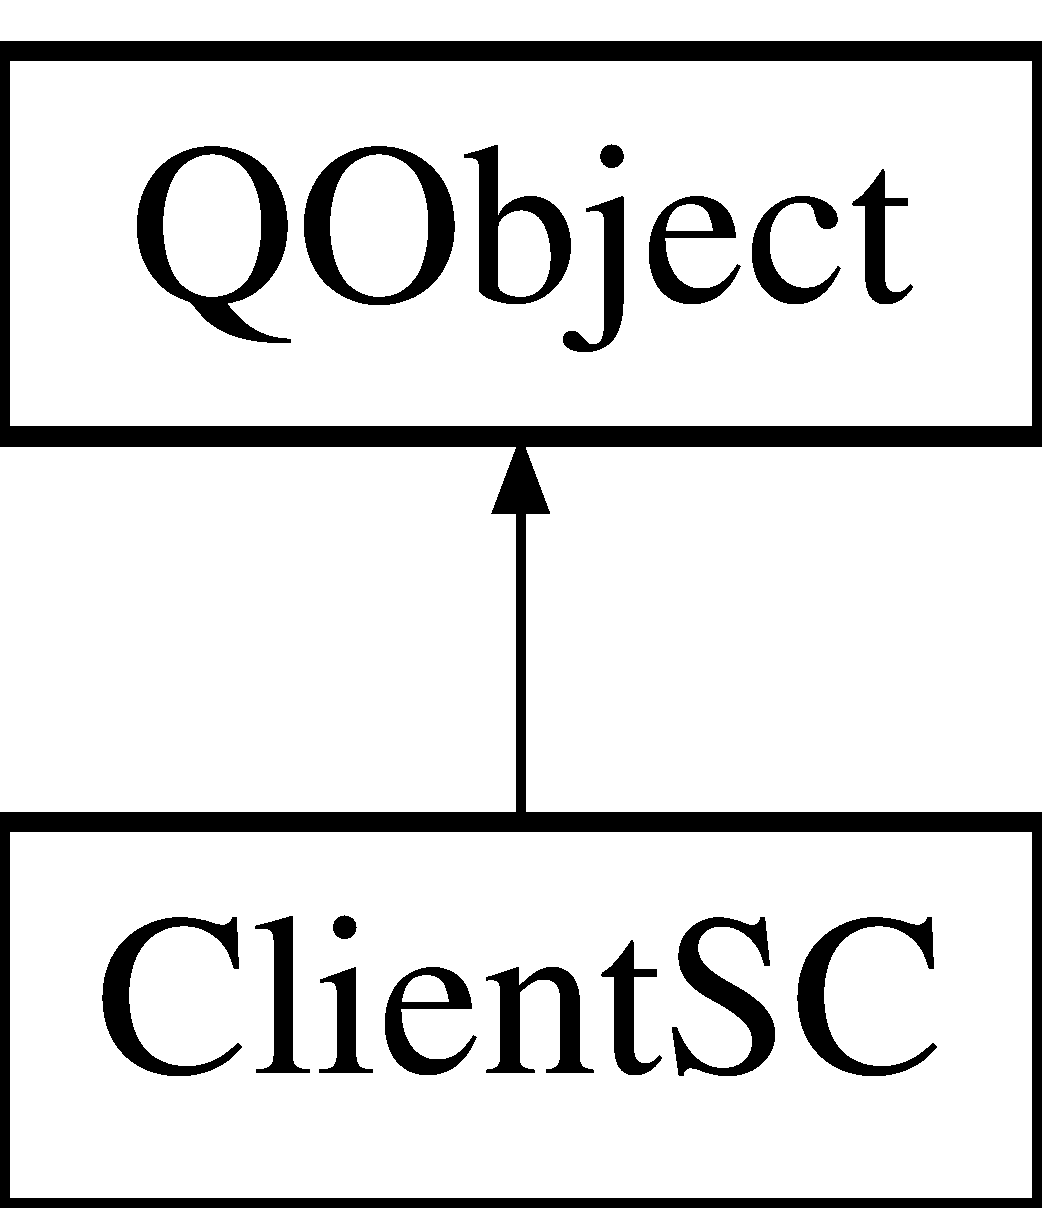
\includegraphics[height=2.000000cm]{classClientSC}
\end{center}
\end{figure}
\subsection*{Signals}
\begin{DoxyCompactItemize}
\item 
void \hyperlink{classClientSC_a88166f0660ddf616b7e26fd5856d907e}{connection\+Established} (int)
\begin{DoxyCompactList}\small\item\em \mbox{[}Signal\mbox{]} connection state \end{DoxyCompactList}\item 
void \hyperlink{classClientSC_ace7df795354f0ddc5ecca1193b0e11b6}{values\+Acquired} (int, float, float, float)
\begin{DoxyCompactList}\small\item\em \mbox{[}Signal\mbox{]} new sensor values have been acquired \end{DoxyCompactList}\item 
void \hyperlink{classClientSC_a0d3a0a5d9496dd2c013a1c9b802dedcb}{send\+Message} (Q\+String)
\begin{DoxyCompactList}\small\item\em \mbox{[}Signal\mbox{]} send a bluetooth message \end{DoxyCompactList}\end{DoxyCompactItemize}
\subsection*{Public Member Functions}
\begin{DoxyCompactItemize}
\item 
\hyperlink{classClientSC_a1333a55122e64b2ef82b7ac1770a66ba}{Client\+SC} ()\hypertarget{classClientSC_a1333a55122e64b2ef82b7ac1770a66ba}{}\label{classClientSC_a1333a55122e64b2ef82b7ac1770a66ba}

\begin{DoxyCompactList}\small\item\em \hyperlink{classClientSC}{Client\+SC} constructor. \end{DoxyCompactList}\item 
void \hyperlink{classClientSC_ae778a4a0aa9805536bc5fbac6d450916}{Connect\+To\+Server} ()\hypertarget{classClientSC_ae778a4a0aa9805536bc5fbac6d450916}{}\label{classClientSC_ae778a4a0aa9805536bc5fbac6d450916}

\begin{DoxyCompactList}\small\item\em Method that starts a discovery and connect to the server when the good service is found. \end{DoxyCompactList}\item 
void \hyperlink{classClientSC_a867af609c1950ada2a6ce6f808b80e81}{Get\+Sensor} (int, int)\hypertarget{classClientSC_a867af609c1950ada2a6ce6f808b80e81}{}\label{classClientSC_a867af609c1950ada2a6ce6f808b80e81}

\begin{DoxyCompactList}\small\item\em Method used to tell server which sensor we want. \end{DoxyCompactList}\item 
void \hyperlink{classClientSC_a66b5a7e9b4de881bc0f77ac973e9a5b9}{Stop\+Client} ()\hypertarget{classClientSC_a66b5a7e9b4de881bc0f77ac973e9a5b9}{}\label{classClientSC_a66b5a7e9b4de881bc0f77ac973e9a5b9}

\begin{DoxyCompactList}\small\item\em Method used to stop the client. \end{DoxyCompactList}\end{DoxyCompactItemize}


\subsection{Member Function Documentation}
\index{Client\+SC@{Client\+SC}!connection\+Established@{connection\+Established}}
\index{connection\+Established@{connection\+Established}!Client\+SC@{Client\+SC}}
\subsubsection[{\texorpdfstring{connection\+Established}{connectionEstablished}}]{\setlength{\rightskip}{0pt plus 5cm}void Client\+S\+C\+::connection\+Established (
\begin{DoxyParamCaption}
\item[{int}]{}
\end{DoxyParamCaption}
)\hspace{0.3cm}{\ttfamily [signal]}}\hypertarget{classClientSC_a88166f0660ddf616b7e26fd5856d907e}{}\label{classClientSC_a88166f0660ddf616b7e26fd5856d907e}


\mbox{[}Signal\mbox{]} connection state 


\begin{DoxyParams}{Parameters}
{\em int} & \+: 0 = client ready ; 1 = Connected ; -\/1 \+: Error \\
\hline
\end{DoxyParams}
\index{Client\+SC@{Client\+SC}!send\+Message@{send\+Message}}
\index{send\+Message@{send\+Message}!Client\+SC@{Client\+SC}}
\subsubsection[{\texorpdfstring{send\+Message}{sendMessage}}]{\setlength{\rightskip}{0pt plus 5cm}void Client\+S\+C\+::send\+Message (
\begin{DoxyParamCaption}
\item[{Q\+String}]{}
\end{DoxyParamCaption}
)\hspace{0.3cm}{\ttfamily [signal]}}\hypertarget{classClientSC_a0d3a0a5d9496dd2c013a1c9b802dedcb}{}\label{classClientSC_a0d3a0a5d9496dd2c013a1c9b802dedcb}


\mbox{[}Signal\mbox{]} send a bluetooth message 


\begin{DoxyParams}{Parameters}
{\em Q\+String} & \+: message \\
\hline
\end{DoxyParams}
\index{Client\+SC@{Client\+SC}!values\+Acquired@{values\+Acquired}}
\index{values\+Acquired@{values\+Acquired}!Client\+SC@{Client\+SC}}
\subsubsection[{\texorpdfstring{values\+Acquired}{valuesAcquired}}]{\setlength{\rightskip}{0pt plus 5cm}void Client\+S\+C\+::values\+Acquired (
\begin{DoxyParamCaption}
\item[{int}]{, }
\item[{float}]{, }
\item[{float}]{, }
\item[{float}]{}
\end{DoxyParamCaption}
)\hspace{0.3cm}{\ttfamily [signal]}}\hypertarget{classClientSC_ace7df795354f0ddc5ecca1193b0e11b6}{}\label{classClientSC_ace7df795354f0ddc5ecca1193b0e11b6}


\mbox{[}Signal\mbox{]} new sensor values have been acquired 


\begin{DoxyParams}{Parameters}
{\em int} & \+: sensor reference \\
\hline
{\em float} & \+: x value \\
\hline
{\em float} & \+: y value \\
\hline
{\em float} & \+: z value \\
\hline
\end{DoxyParams}


The documentation for this class was generated from the following file\+:\begin{DoxyCompactItemize}
\item 
clientsc.\+h\end{DoxyCompactItemize}

\hypertarget{classFrame3D}{}\section{Frame3D Class Reference}
\label{classFrame3D}\index{Frame3D@{Frame3D}}
Inheritance diagram for Frame3D\+:\begin{figure}[H]
\begin{center}
\leavevmode
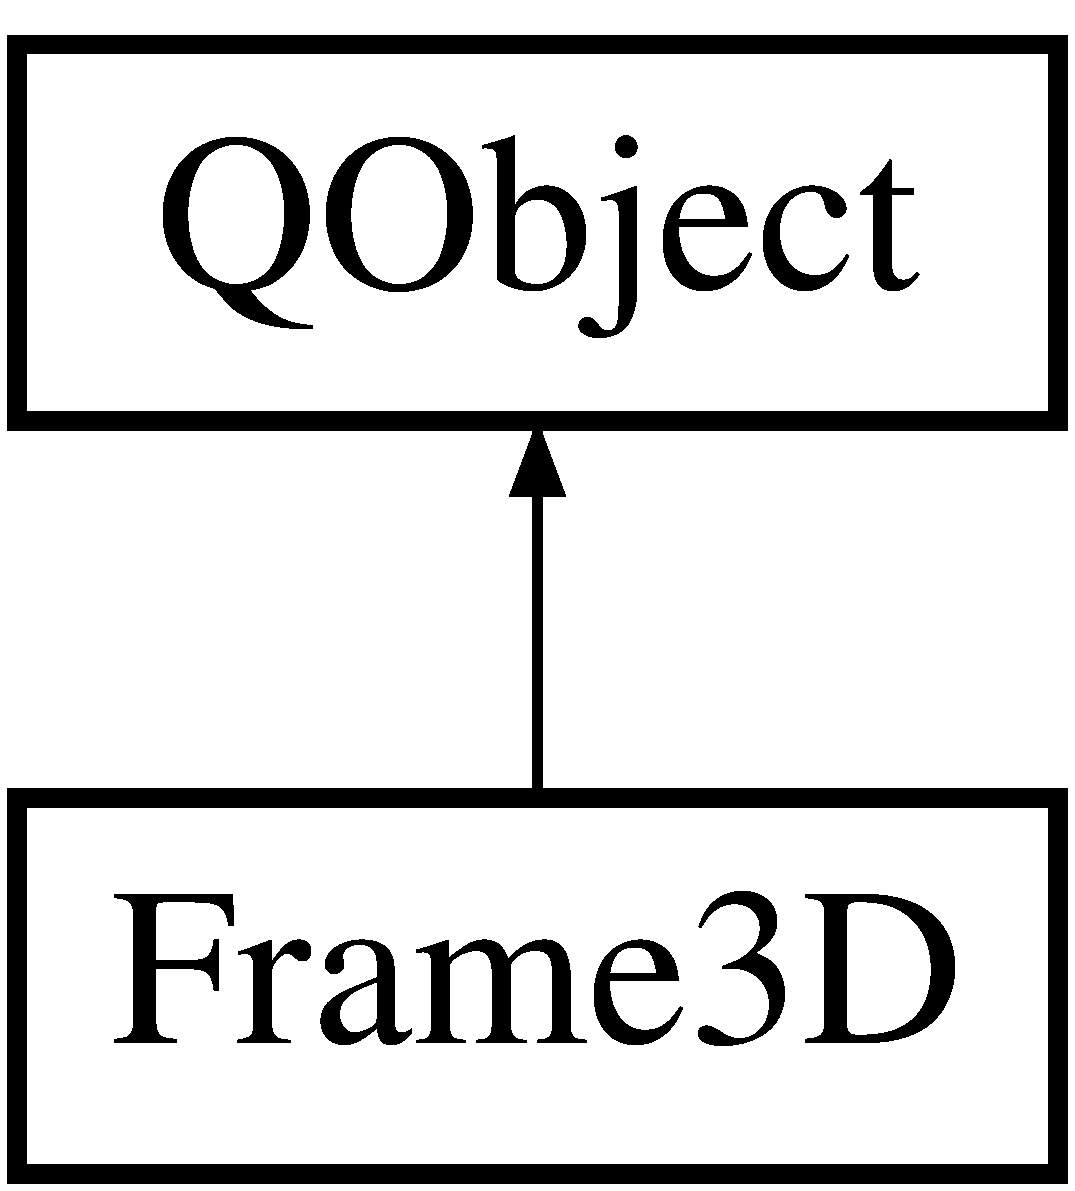
\includegraphics[height=2.000000cm]{classFrame3D}
\end{center}
\end{figure}
\subsection*{Public Slots}
\begin{DoxyCompactItemize}
\item 
void {\bfseries rotate} (float x, float y, float z)\hypertarget{classFrame3D_a19be0f7e71a530ea1c80986ce7a827c6}{}\label{classFrame3D_a19be0f7e71a530ea1c80986ce7a827c6}

\item 
void {\bfseries calibrate} ()\hypertarget{classFrame3D_ab1b21cf60fcbee4957b42319964228e1}{}\label{classFrame3D_ab1b21cf60fcbee4957b42319964228e1}

\end{DoxyCompactItemize}


The documentation for this class was generated from the following files\+:\begin{DoxyCompactItemize}
\item 
frame3d.\+h\item 
frame3d.\+cpp\end{DoxyCompactItemize}

\hypertarget{classMainWindow}{}\section{Main\+Window Class Reference}
\label{classMainWindow}\index{Main\+Window@{Main\+Window}}
Inheritance diagram for Main\+Window\+:\begin{figure}[H]
\begin{center}
\leavevmode
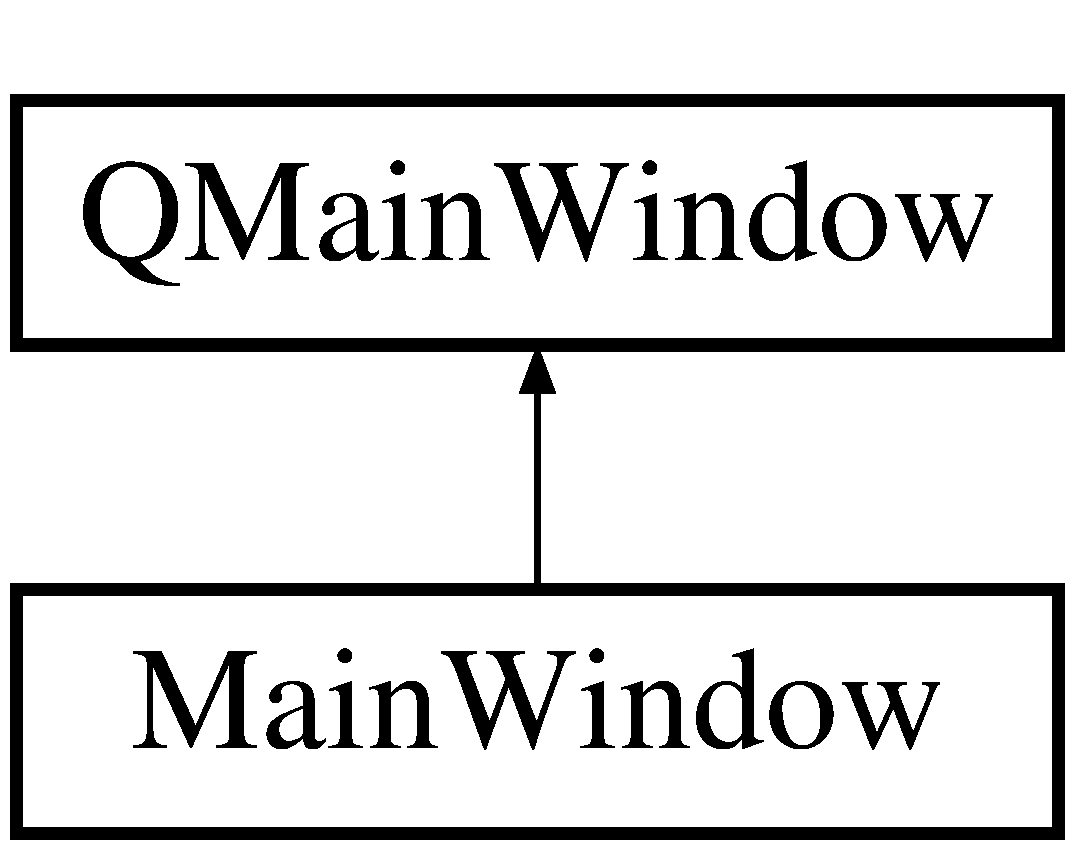
\includegraphics[height=2.000000cm]{classMainWindow}
\end{center}
\end{figure}
\subsection*{Signals}
\begin{DoxyCompactItemize}
\item 
void {\bfseries send\+Message} (const Q\+String \&message)\hypertarget{classMainWindow_a35c45a6273f5cfff11a110bfeafdbb7f}{}\label{classMainWindow_a35c45a6273f5cfff11a110bfeafdbb7f}

\end{DoxyCompactItemize}
\subsection*{Public Member Functions}
\begin{DoxyCompactItemize}
\item 
{\bfseries Main\+Window} (Q\+Widget $\ast$parent=0)\hypertarget{classMainWindow_a8b244be8b7b7db1b08de2a2acb9409db}{}\label{classMainWindow_a8b244be8b7b7db1b08de2a2acb9409db}

\item 
void {\bfseries debug} (Q\+String msg)\hypertarget{classMainWindow_aac864c0d1dc51d589bc61ae68c6a0297}{}\label{classMainWindow_aac864c0d1dc51d589bc61ae68c6a0297}

\end{DoxyCompactItemize}


The documentation for this class was generated from the following files\+:\begin{DoxyCompactItemize}
\item 
Main\+Window.\+h\item 
Main\+Window.\+cpp\end{DoxyCompactItemize}

\hypertarget{classServerSC}{}\section{Server\+SC Class Reference}
\label{classServerSC}\index{Server\+SC@{Server\+SC}}
Inheritance diagram for Server\+SC\+:\begin{figure}[H]
\begin{center}
\leavevmode
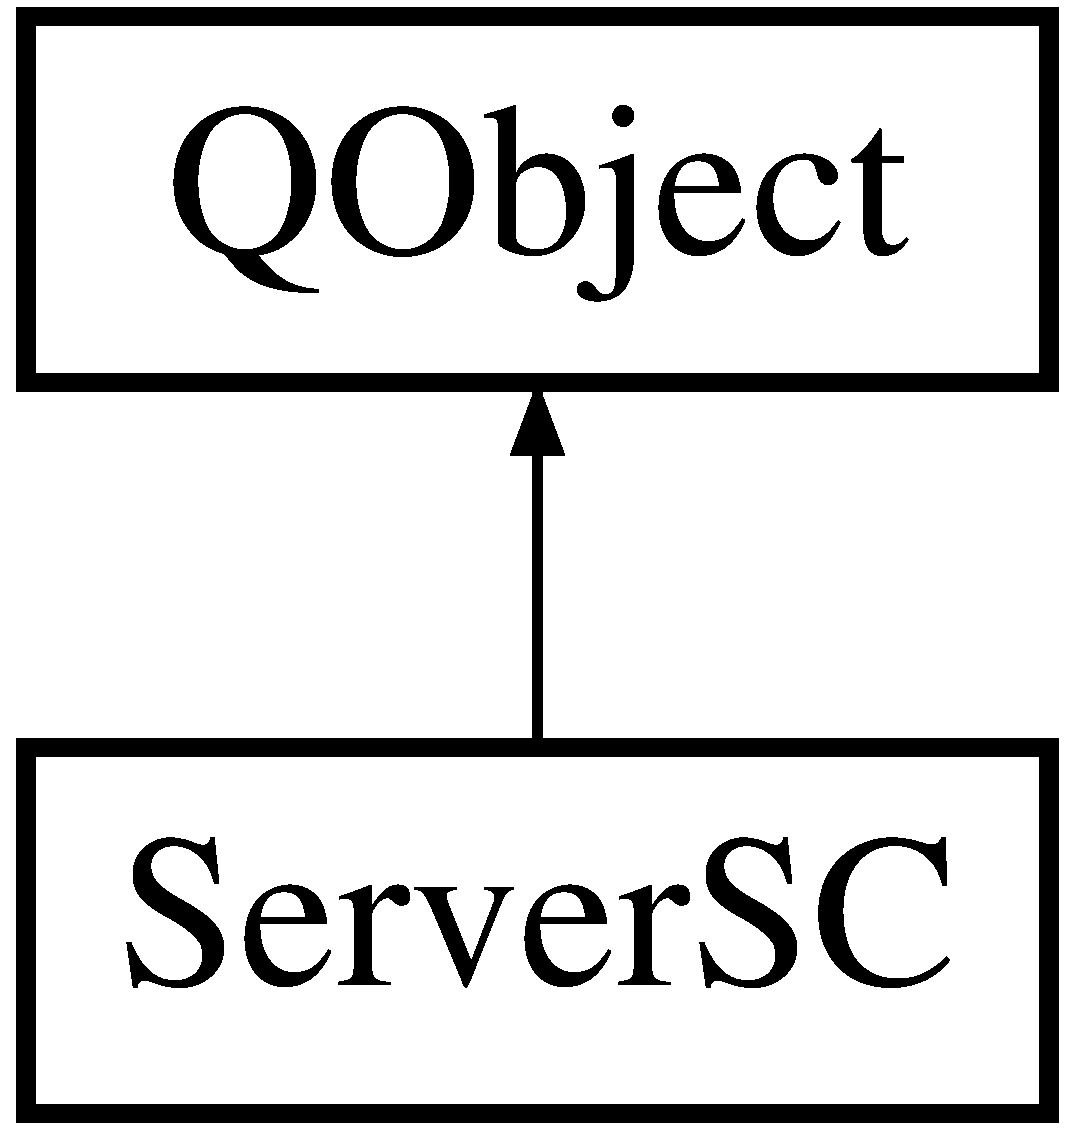
\includegraphics[height=2.000000cm]{classServerSC}
\end{center}
\end{figure}
\subsection*{Signals}
\begin{DoxyCompactItemize}
\item 
void \hyperlink{classServerSC_aa2c6d7cead4892c210a2c2a535f8f00e}{connection\+Established} (int)\hypertarget{classServerSC_aa2c6d7cead4892c210a2c2a535f8f00e}{}\label{classServerSC_aa2c6d7cead4892c210a2c2a535f8f00e}

\begin{DoxyCompactList}\small\item\em Signal emitted to. \end{DoxyCompactList}\item 
void {\bfseries send\+Message} (Q\+String)\hypertarget{classServerSC_a939f52aa74d902207ef986b4e01d46cd}{}\label{classServerSC_a939f52aa74d902207ef986b4e01d46cd}

\item 
void {\bfseries s\+\_\+debug} (Q\+String)\hypertarget{classServerSC_ac8855e3bdddb9a31c127678404673829}{}\label{classServerSC_ac8855e3bdddb9a31c127678404673829}

\end{DoxyCompactItemize}
\subsection*{Public Member Functions}
\begin{DoxyCompactItemize}
\item 
void \hyperlink{classServerSC_a52e32a2100f99d8b6c16ffece88ee633}{Start\+Server} ()\hypertarget{classServerSC_a52e32a2100f99d8b6c16ffece88ee633}{}\label{classServerSC_a52e32a2100f99d8b6c16ffece88ee633}

\begin{DoxyCompactList}\small\item\em Demarrer le serveur. \end{DoxyCompactList}\item 
void \hyperlink{classServerSC_a1272d2b6654fcaa3668f02cdac58846d}{Stop\+Server} ()\hypertarget{classServerSC_a1272d2b6654fcaa3668f02cdac58846d}{}\label{classServerSC_a1272d2b6654fcaa3668f02cdac58846d}

\begin{DoxyCompactList}\small\item\em Stopper le serveur. \end{DoxyCompactList}\end{DoxyCompactItemize}


The documentation for this class was generated from the following file\+:\begin{DoxyCompactItemize}
\item 
serversc.\+h\end{DoxyCompactItemize}

\hypertarget{classWindow}{}\section{Window Class Reference}
\label{classWindow}\index{Window@{Window}}
Inheritance diagram for Window\+:\begin{figure}[H]
\begin{center}
\leavevmode
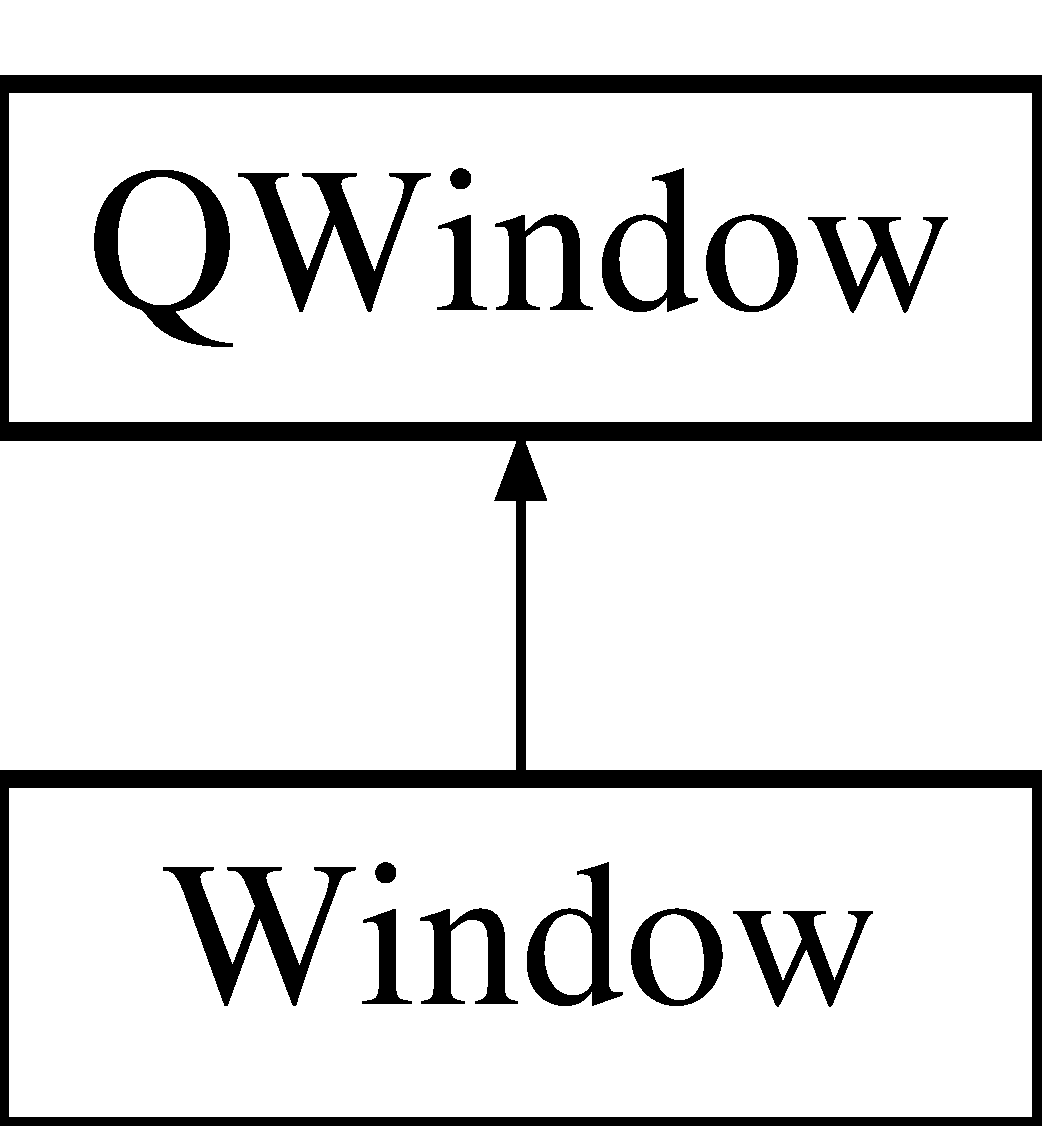
\includegraphics[height=2.000000cm]{classWindow}
\end{center}
\end{figure}
\subsection*{Signals}
\begin{DoxyCompactItemize}
\item 
void {\bfseries calibrate} ()\hypertarget{classWindow_a83e2ec02725fb17ac682b7de4a09f8d8}{}\label{classWindow_a83e2ec02725fb17ac682b7de4a09f8d8}

\end{DoxyCompactItemize}
\subsection*{Public Member Functions}
\begin{DoxyCompactItemize}
\item 
{\bfseries Window} (Q\+Screen $\ast$screen=0)\hypertarget{classWindow_aca6dcd6e39eeb5284f8dea2cf22e3977}{}\label{classWindow_aca6dcd6e39eeb5284f8dea2cf22e3977}

\end{DoxyCompactItemize}
\subsection*{Protected Member Functions}
\begin{DoxyCompactItemize}
\item 
virtual void {\bfseries key\+Press\+Event} (Q\+Key\+Event $\ast$e)\hypertarget{classWindow_a5d729d5dc8bf34c67de323555f173b8f}{}\label{classWindow_a5d729d5dc8bf34c67de323555f173b8f}

\end{DoxyCompactItemize}


The documentation for this class was generated from the following files\+:\begin{DoxyCompactItemize}
\item 
window.\+h\item 
window.\+cpp\end{DoxyCompactItemize}

%--- End generated contents ---

% Index
\backmatter
\newpage
\phantomsection
\clearemptydoublepage
\addcontentsline{toc}{chapter}{Index}
\printindex

\end{document}
